\section{Prototypical Service Mesh Setup}

The following chapter describes our concept of our prototypical service mesh implementation and its outcome. In order to also practically work out the differences between service meshes and a traditional microservice operation, we will initially run our application using only \kubernetes{}, and then later set up a service mesh.

\begin{figure*}
    \centering
    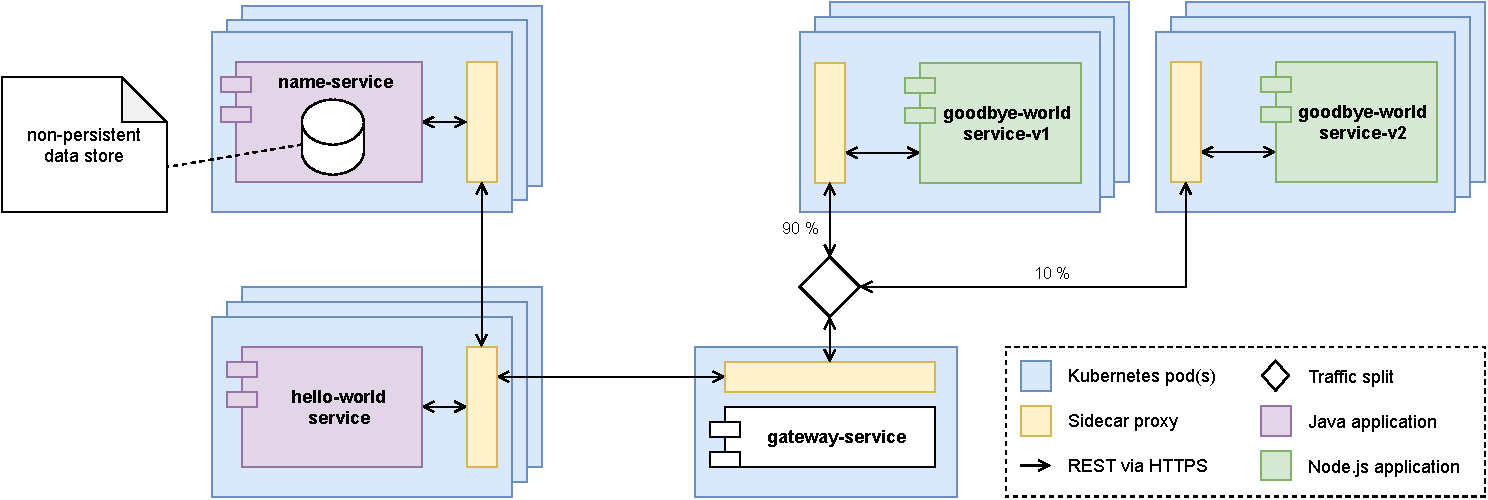
\includegraphics[width=\textwidth]{img/diagram-draft.pdf}
    \caption{Architecture overview of the PoC application}
    \label{fig:poc-overview}
\end{figure*}

\subsection{Services}
\label{sec:services}

Our basic idea is to implement three simple microservice applications that communicate via REST. To prove technology independence, one service is written in Node.js, while the other two services are written in Python. Another requirement to meet is that the services have to be as simple as possible. Furthermore, the functionality of the services is intended to be as follows:

\begin{itemize}
\item \textsc{name-service}: Provides endpoint to retrieve a collection of names. It stores the names in a file or a simple array list.
\item \textsc{goodbye-world-service}: Provides endpoint to retrieve a message ``Goodbye, World!"
\item \textsc{hello-world-service}: Contacts the \textsc{name-service} and provides an endpoint that returns a ``Hello, \{name\}" message for each name object from name service.
\end{itemize}

Since Linkerd does not provide an own ingress controller (see chapter \ref{linkerd}), we use an external ingress controller named \textsc{traefik}.

\subsection{Showcases}
\label{sec:showcases-1}

Our prototypical implementation aims to provide answers to the following five challenges of running and maintaining microservices.

\subsubsection{Encryption}

By using a service mesh, it should be shown that an encryption policy can be easily applied or removed.

\subsubsection{Canary Deployment}

To provide an example showcase for canary deployment, we implemented two versions of \textsc{name-service} which differ by the returned string (version 1 returns only forename while version 2 returns surname as well).
The mesh is tasked with redirecting traffic so that 90\% of all requests are made to version 1 and 10\% of requests are made to version 2.

\subsubsection{Access Policies}

Another restriction is that the \textsc{name-service} is only accessible from the \textsc{hello-world-service}. Access restriction should not be a task of the actual \textsc{name-service} application. We want to show that access to services is easily managable via YAML resources.


\subsubsection{Load Balancing}
TBD

\subsubsection{Central Monitoring and Logging}
The proof of concept should show that services in a microservice landscape can be monitored and managed centrally using the service mesh.

\subsection{Setup of Linkerd}

The following sequence of bash commands shows the \textsc{Linkerd} installation process and the application of the service mesh to the \textsc{Kubernetes} cluster \cite{linkerd-get-started}:
\begin{lstlisting}[language=bash,caption={Setup of \textsc{Linkerd}}, label={lst:linkerd-setup}]
#!/bin/bash
curl -sL https://run.linkerd.io/install \
	| sh
echo "export PATH=$PATH:~/.linkerd2/bin" \
	>> ~/.bashrc
linkerd install | kubectl apply -f -
\end{lstlisting}
The first line downloads and runs the install-script which chooses the correct installation for running operating system and validates checksum before finally linking the executable for \linkerd{}-CLI.
The second line exports installation path of \linkerd{} into the \lstinline|$PATH|-environment. 
Finally line 3 uses the \linkerd{}-CLI and installs the control plane on the cluster.
\lstinline|linkerd install| returns a \kubernetes{} manifest in YAML, which is "piped" into \lstinline|kubectl| to apply all contained control plane resources.

From now the framework for our service mesh is done.
All communication between \linkerd{}-proxies are encrypted by default.

You may notice the use of the "pipe". 
This is a usual workflow in \linkerd{}: The output is a YAML-file, that can be piped into \lstinline|kubectl|.

\subsection{Adding Services into Linkerd}
Until now the service mesh is ruled only by \linkerd{}s own services.
To add a service, you start with a common \kubernetes{}-manifest in YAML.
But instead of giving it to \lstinline|kubectl| directly, you "inject" a \linkerd{} command showed in \autoref{lst:linkerd-inject}.
\begin{lstlisting}[language=bash,caption={Inject \textsc{Linkerd}-annotation into manifest.}, label={lst:linkerd-inject}]
cat <config-yml> \
	| linkerd inject - \
	| kubectl apply -f -
\end{lstlisting}
Since \linkerd{}-CLI is in between these command, \lstinline|inject| parses the YAML and adds annotations to it.
The annotated file is passed into \lstinline|kubectl| in the common way.
\linkerd{}-CLI searches for deployments to annotate.
This way all Services belonging to one deployment can be covered.
\autoref{lst:linkerd-annotation} shows an extract of an annotated YAML file.
It says, \linkerd{} will inject every Pod in this deployment with its proxies.

\begin{lstlisting}[caption={Extract of a \kubernetes{}-manifest annotated by \textsc{Linkerd}.}, label={lst:linkerd-annotation}]
kind: Deployment
spec:
[...]
	template:
		metadata:
			annotations:
				linkerd.io/inject: enabled
[...]				
\end{lstlisting}
 
\subsection{Communication between Services}

In the \kubernetes{}-manifest the names of cluster, namespace and service is defined.
From this the unique DNS-name is derived the following way:

\begin{lstlisting}[caption={DNS-name of a local service in \kubernetes{}.}, label={lst:k8s-dns}]
<svc-name>.<namespace>.svc.<cluster>.local
\end{lstlisting}

When calling this DNS-name, \kubernetes{} will dissolve corresponding Pod and redirect the request accordingly.
This way an application A can easily access the API of an application B within the same cluster under its DNS-name.
And this holds even with service mesh.
\linkerd{} wraps each application into a Pod next to \linkerd{}-proxy.
Communication between Services is now routed via these proxies through the service mesh.
But from the view of the application it works the same way as before.

\subsection{\traefik{} as Ingress Controller}

How do we reach our services from outside?
Therefore we need an ingress controller.
As stated in \autoref{linkerd} we chose \traefik{}.
Sure, \traefik{} could cope quite more than an ingress, but we will only use its remote proxy functionality here.
\autoref{lst:ingress-hello} shows the configuration file for the ingress route \lstinline|/helloworld| to the corresponding \textsc{hello-world-service} as stated in \autoref{sec:services}.
Again the interesting part is in the metadata annotation.
First we tell \kubernetes{} to use \traefik{} as ingress controller.
Second we route all traffic to the corresponding \linkerd{}-sidecar (abbreviated here in \kubernetes{}-style with \lstinline|l5d|).
This configuration allows us to use different routes for different services by calling another path in the URL.
Analog route we defined for \textsc{goodbye-world-service}.

\begin{lstlisting}[caption={YAML configuration of \lstinline|helloworld|-ingress controller.}, label={lst:ingress-hello}]]
apiVersion: extensions/v1beta1
kind: Ingress
metadata:
	name: helloworld
	annotations:
		kubernetes.io/ingress.class: "traefik"
		ingress.kubernetes.io/
			custom-request-headers: 
			l5d-dst-override:helloworld.default
			.svc.cluster.local:80
spec:
	rules:
	- http:
		paths:
		- path: /helloworld
			backend:
			serviceName: helloworld
			servicePort: 80
\end{lstlisting}

Now that the infrastructure is in place, we care about implementation of the showcases.

%\subsection{Resource Definition for Applications}

%\subsection{Policy Application}